
\documentclass[10pt,a4paper]{article}
    \usepackage[utf8]{inputenc}
    \usepackage{xcolor}
    % \usepackage[utf8x]{inputenc} % para poder usar tildes en archivos UTF-8
    \usepackage[spanish,es-tabla]{babel}
    \usepackage{verbatim}
    \usepackage{clrscode3e}
    \usepackage{amssymb}
    \usepackage{amsmath}
    \usepackage{amsfonts} % for the \checkmark command 
    \usepackage{graphicx}
    \usepackage{float}
    \usepackage{pdfpages}
    \usepackage{enumerate}
    \usepackage{caption}
    \usepackage{subcaption}
    \usepackage[left=3cm, right=3cm, top=2cm]{geometry}
% \documentclass[10pt,a4paper]{article}
% \usepackage[utf8x]{inputenc} % para poder usar tildes en archivos UTF-8
% \usepackage[spanish,es-tabla]{babel}
% \usepackage{verbatim}
% \usepackage{amsmath}
% \usepackage{clrscode3e}
% \usepackage{amssymb}
% \usepackage{graphicx}
% \usepackage{float}
% \usepackage{pdfpages}

%\usepackage{bibtex}

%\usepackage{a4wide} % márgenes un poco más anchos que lo usual

\usepackage{caratula} % Se puede descargar en ~> https://github.com/bcardiff/dc-tex
\usepackage[breaklinks=true]{hyperref}


\begin{document} % Todo lo que escribamos a partir de aca va a aparecer en el documento.

%fran
%\sloppy

% Completar los datos de la caratula
\titulo{Trabajo Práctico 2}
\fecha{\today}
\materia{Algoritmos y Estructuras Datos III}
\grupo{Grupo ``Apruebennos que Santi es de Racing''}

% Completar los integrantes del grupo:)
\integrante{Cristian Kubrak}{456/15}{kubrakcristian@gmail.com}
\integrante{Santiago Feliu}{644/15}{santiagofeliu@gmail.com}
\integrante{Pablo Ingaramo}{544/15}{pablo2martin@hotmail.com}
\integrante{Kennedy William Rios Cuba}{503/15}{wrios@dc.uba.ar}

\maketitle 

% \par \textbf{Abstract:} El objetivo de este trabajo es resolver el problema de la suma de
% subconjuntos mediante 3 diferentes t\'ecnicas: Fuerza Bruta, Backtracking y 
% Programaci\'on din\'amica para luego analizar cu\'al de ellas resulta mejor aplicar seg\'un el contexto.

\tableofcontents
% \par  \textbf{Palabras clave:} subset sum - brute force - Backtracking - Programaci\'on din\'amica
% Aca comienzan a escribir su informe


\newpage

\section{Introducción}
\par A continuaci\'on se busca resolver el problema del \textit{arbitraje}: dado un mercado de divisas se busca
obtener ganancia a partir de comprar y vender divisas en simultaneo de manera de aprovechar desbalances 
en el mercado. Estos desbalances no suelen suceder de manera inmediata (obtener ganancia ante la compra/venta
de una sola divisa), raz\'on por la cual hay que realizar un recorrido de varias divisas a modo de obtener ganacias.
\par Interpretamos los precios de compra/venta como un digrafo completo donde el peso
de la arista que une a la divisa \textit{i} con la divisa \textit{j} representa el multiplicador 
que se debe aplicar a una unidad de la divisa \textit{i} al cambiar a la divisa \textit{j}.
\par Sea $W_{ij}$ la matriz de adyacencias, $(W')_{ij} = - \log (w_{ij})$, y teniendo en 
cuenta que \textbf{(CITAR DEMO)}
\begin{equation}
    \log{ (\prod_{i=1}^n a_i}) = \sum_{i=1}^n (\log{ a_i})
\end{equation}
\par nos dimos cuenta que resolver el problema de obtener ganacias equivale a encontrar ciclos negativos en
$(W')_{ij}$.
\par Para encontrar ciclos negativos decidimos usar y comparar dos algoritmos: el de Bellman-Ford y el de
FloyWarshall. A cada uno de estos tuvimos que agregarle una forma distinta de recontruir el ciclo negativo.

\subsubsection{Ejemplos}

\textbf{Ejemplo con ciclos}\\
Sea $(W)_{ij}$ la matriz de adyacencias definida como:
    
\begin{figure}[H] 
    \centering
    \begin{minipage}{0.35\textwidth}
        \centering
\[
W=
  \begin{bmatrix}
    1 & 2 & 1 & 1\\
    2 & 2 & 2 & 1\\
    2 & 1 & 1 & 2\\
    2 & 1 & 1 & 1
  \end{bmatrix}
\]
    \end{minipage}
    \begin{minipage}{0.45\textwidth}
        \centering
\[
W'=
  \begin{bmatrix}
    0 & -0.30 & 0 & 0\\
    -0.30 & -0.30 & -0.30 & 0\\
    -0.30 & 0 & 0 & -0.30\\
    -0.30 & 0 & 0 & 0
  \end{bmatrix}
\]
    \end{minipage}\hfill
\end{figure}


\begin{figure}[H] 
\centering
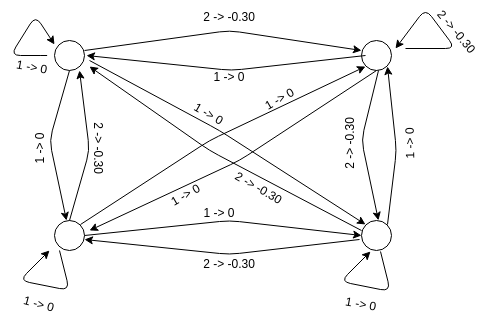
\includegraphics[width=.5\textwidth]{img/grafobase.png}
\caption{Grafo resultante de $(W)_{ij}$ y $(W')_{ij}$}
\label{fig:grafobaseconciclos}
\end{figure}

\begin{figure}[H] 
    \centering
    \begin{minipage}{0.45\textwidth}
        \centering
        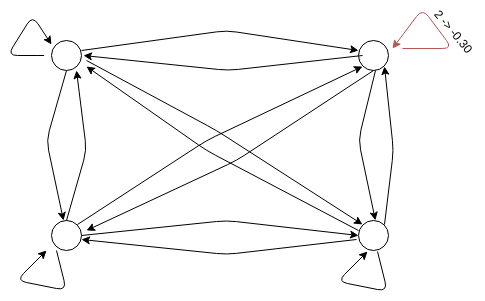
\includegraphics[width=1\textwidth]{img/ccciclosimple.png} % first figure itself
        \caption{Ciclo negativo de un solo elemento}
        \label{fig:ciclouno}
    \end{minipage}\hfill
    \begin{minipage}{0.45\textwidth}
        \centering
        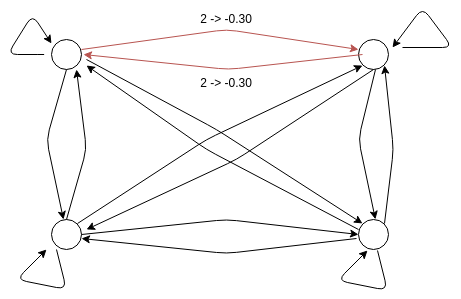
\includegraphics[width=1\textwidth]{img/ccciclodoble.png} % first figure itself
        \caption{Ciclo negativo de dos elementos}
        \label{fig:ciclodos}
    \end{minipage}\hfill
\end{figure}

\begin{figure}[H] 
    \centering
    \begin{minipage}{0.45\textwidth}
        \centering
        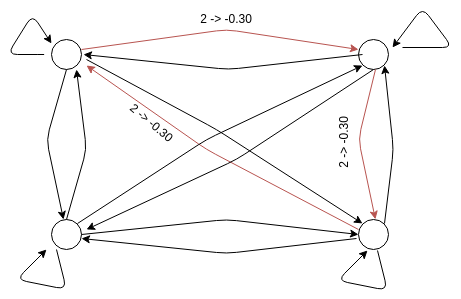
\includegraphics[width=1\textwidth]{img/ccctriple.png} % first figure itself
        \caption{Ciclo negativo de tres elementos}
        \label{fig:ciclotres}
    \end{minipage}\hfill
    \begin{minipage}{0.45\textwidth}
        \centering
        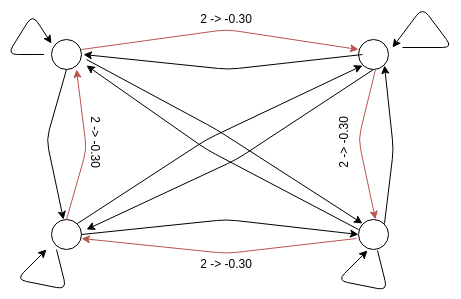
\includegraphics[width=1\textwidth]{img/ccciclocuatro.png} % first figure itself
        \caption{Ciclo negativo de cuatro elementos}
        \label{fig:ciclocuatro}
    \end{minipage}\hfill
\end{figure}

En las figuras \ref{fig:ciclouno}, \ref{fig:ciclodos}, \ref{fig:ciclotres} y \ref{fig:ciclocuatro} se obtienen un ciclos
negativos de valor $-0.3$, $-0.6$, $-0.9$ y $-1.2$ lo cual se traduce en ganacias del $100\%$, $200\%$, $300\%$ y $400\%$
de la unidad con la que se empieza. Para los alcances de este trabajo nos alcanza con que los algoritmos en cuesti\'on
devuelan cualquiera de estos ciclos.

\textbf{Ejemplo sin ciclos}\\
Sea $(W)_{ij}$ la matriz de adyacencias definida como:
    
\begin{figure}[H] 
    \centering
    \begin{minipage}{0.35\textwidth}
        \centering
\[
W=
  \begin{bmatrix}
    1 & 2 & 3 \\
    0.5 & 1 & 2 \\
    0.25 & 0.5 & 1
  \end{bmatrix}
\]
    \end{minipage}
    \begin{minipage}{0.45\textwidth}
        \centering
\[
W'=
  \begin{bmatrix}
    0 & -0.30 & 0.60 \\
    -0.30 & 0 & 0.30 \\
    -0.60 & -0.30 & 0
  \end{bmatrix}
\]
    \end{minipage}\hfill
\end{figure}


\begin{figure}[H] 
\centering
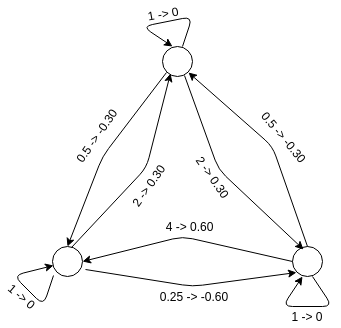
\includegraphics[width=.3\textwidth]{img/sinCiclos.png}
\caption{Grafo resultante de $(W)_{ij}$ y $(W')_{ij}$}
\label{fig:grafobaseconciclos}
\end{figure}

En este caso no existen ciclos negativos en $(W')_{ij}$ lo cual se traduce en que no existen posibilidades de arbitraje.
\newpage

\section{Desarrollo}
\par Comenzamos con la matriz de adyacencia $(W)_{ij}$ que luego transformamos en $(W')_{ij}$ donde $w'_{ij} = - \log w_{ij}$
\par Tal como mencionamos previamente, creamos esta nueva matriz para que poder encontrar una soluci\'on al problema
del arbitraje se limite a hallar ciclos negativos.
\par No solo nos importa decidir si existe o no un ciclo negativo, sino que tambi\'en nos interesa poder reconstruirlo
(ese ser\'a la sucesi\'on de compra/venta de divisas que deber\'iamos realizar para obtener gananacia). 
Para esto utilizamos variantes de dos algoritmos.
\subsubsection{Floyd-Warshall}
Para encontrar un ciclo negativo, utilizamos en escencia el algoritmo de Floyd-Warshall solo que agregando algunas
cosas:
\begin{enumerate}
\item Contamos tambi\'en con una matriz de $nxn$ en el cual guardamos los nodos siguientes al que estamos recorriendo.
\item A la hora de actualizar la matriz de distancias, tambi\'en actualizamos la de nodos siguientes.
\item Una vez finalizadas el algoritmo de FW, revisamos si alg\'un elemento en la diagonal de distancias es negativo
(esto implica que existe un ciclo negativo).
\end{enumerate}
Sea $i$ el nodo en el cual encontramos un ciclo negativo ($distancias[i][i] < 0$)

\begin{codebox}
    \Procname {\proc{CicloNegativo}(Matriz($int$) $siguientes$, int $i$)}
    \li $recorrido$.agregar($i$)
    \li $v = i$
    \li $u$ = $siguientes[u][v]$
    \li \While ($u \neq v$)
        \Then
    \li     $recorrido$.agregar($u$)
    \li     $u$ = $siguiente[u][v]$
    \End
    \li $recorrido$.agregar($i$)
    \li \Return $recorrido$
\end{codebox}

\par A la hora de analizar la complejidad de esta variaci\'on de Floyd-Warshall partimos de la base que FW tiene una complejidad
de $O(n^3)$. Nuestra modificaci\'on solo agrega la creaci\'on de la matriz $siguientes$ ($O(n^2)$) y luego actualizarla 
cada vez que FW actualiza distancias lo cual no afecta la complejidad asint\'otica del algoritmo.
\par Para reconstruir el ciclo negativo, el mismo tendr\'a longitud a lo sumo $n$ raz\'on por la cual la guarda de 
la linea 4 se ejecutar\'a a lo sumo $n$ veces.
\par En conclusi\'on la ejecuci\'on de este algoritmo tendr\'a como complejidad $(O(n^3))$

\subsubsection{Bellman-Ford}
Para encontrar un ciclo negativo, utilizamos en escencia el algoritmo de Bellman-Ford introduciendo algunas
modificaciones para poder reconstruir el ciclo negativo:

\begin{enumerate}
\item Contamos tambi\'en con un vector $predecesor$ en el cual almacenamos el nodo predecesor al que
estamos investigando.
\end{enumerate}

\newpage

\section{Experimentaci\'on}
% \input{experimentacion}
\newpage

\section{Resultados}
% \input{resultados}
\newpage

\section{Conclusiones}
% \input{conclusiones}
\newpage

\section{Ap\'endice}
% \input{apendice}


\end{document}

